\section{Schwankungsbreite}
\label{sec:Schwankungsbreite}
\subsection{j}
Um die Auslegung des Systems zu vollenden, ist es notwendig neben der gemittelten
Variante auch die Extrema zu dimensionieren, um abschließend feststellen zu können, ob
Anpassungen am gemittelten System notwendig sind, um eine sichere Versorgung
gewährleisten zu können.\\
Das erste Extrema ist die Dimensionierung der Anlage bei maximaler Bestrahlung $E_{gen,max}$ und
minimalem jährlichen Gesamtwärmebedarf $Q_{Ges,min}$. Beim zweiten Extrema werden die jeweils entgegengesetzten
Werte genutzt.\\
Das erste Extrema benötigt 2 Kollektoren weniger, da bei höherem Ertrag je Kollektor weniger Wärme benötigt
wird. Es handelt sich also um die in diesem Rahmen bestmöglichen Umstände.
Daraus folgt ebenfalls, dass das Speichervolumen um 231 Liter sinkt und der kleiner Viessmann Vitocell 340-M Speicher
verwendet werden kann. Die Rohrleitung für beide Systeme wären DIN20-Rohre. Das führt dazu, dass der Volumenstrom
im Vergleich sinkt, die Strömung laminar wird und eine Verringerung des Gesamtdruckverlustes um rund 15000 Pa erwartbar ist.\\
Das zweite Extrema stellt insgesamt betrachtet den erwartbaren Worst Case dar.
Es würde 1 Kollektor mehr benötigt werden als beim gemittelten System. Beim Speicher würde weiterhin
der Viessmann Vitocell 360-M mit 950 Liter Fassungsvermögen genutzt werden, obwohl der errechnete Speicherraum
um 115,5 Liter auf 1039,5 Liter steigen würde. Hier gäbe es keine Änderung, da wir bei diesem Modell bereits den größten
Speicher des gewählten Herstellers nutzen. Die Rohrleitungen des Systems müssten auf DIN25 vergrößert werden, so
hätte das System trotz gestiegenem Volumenstrom eine Minderung des Gesamtdruckverlustes von rund 6800 Pa vorzuweisen.\\

\begin{figure}[H]
    \centering
    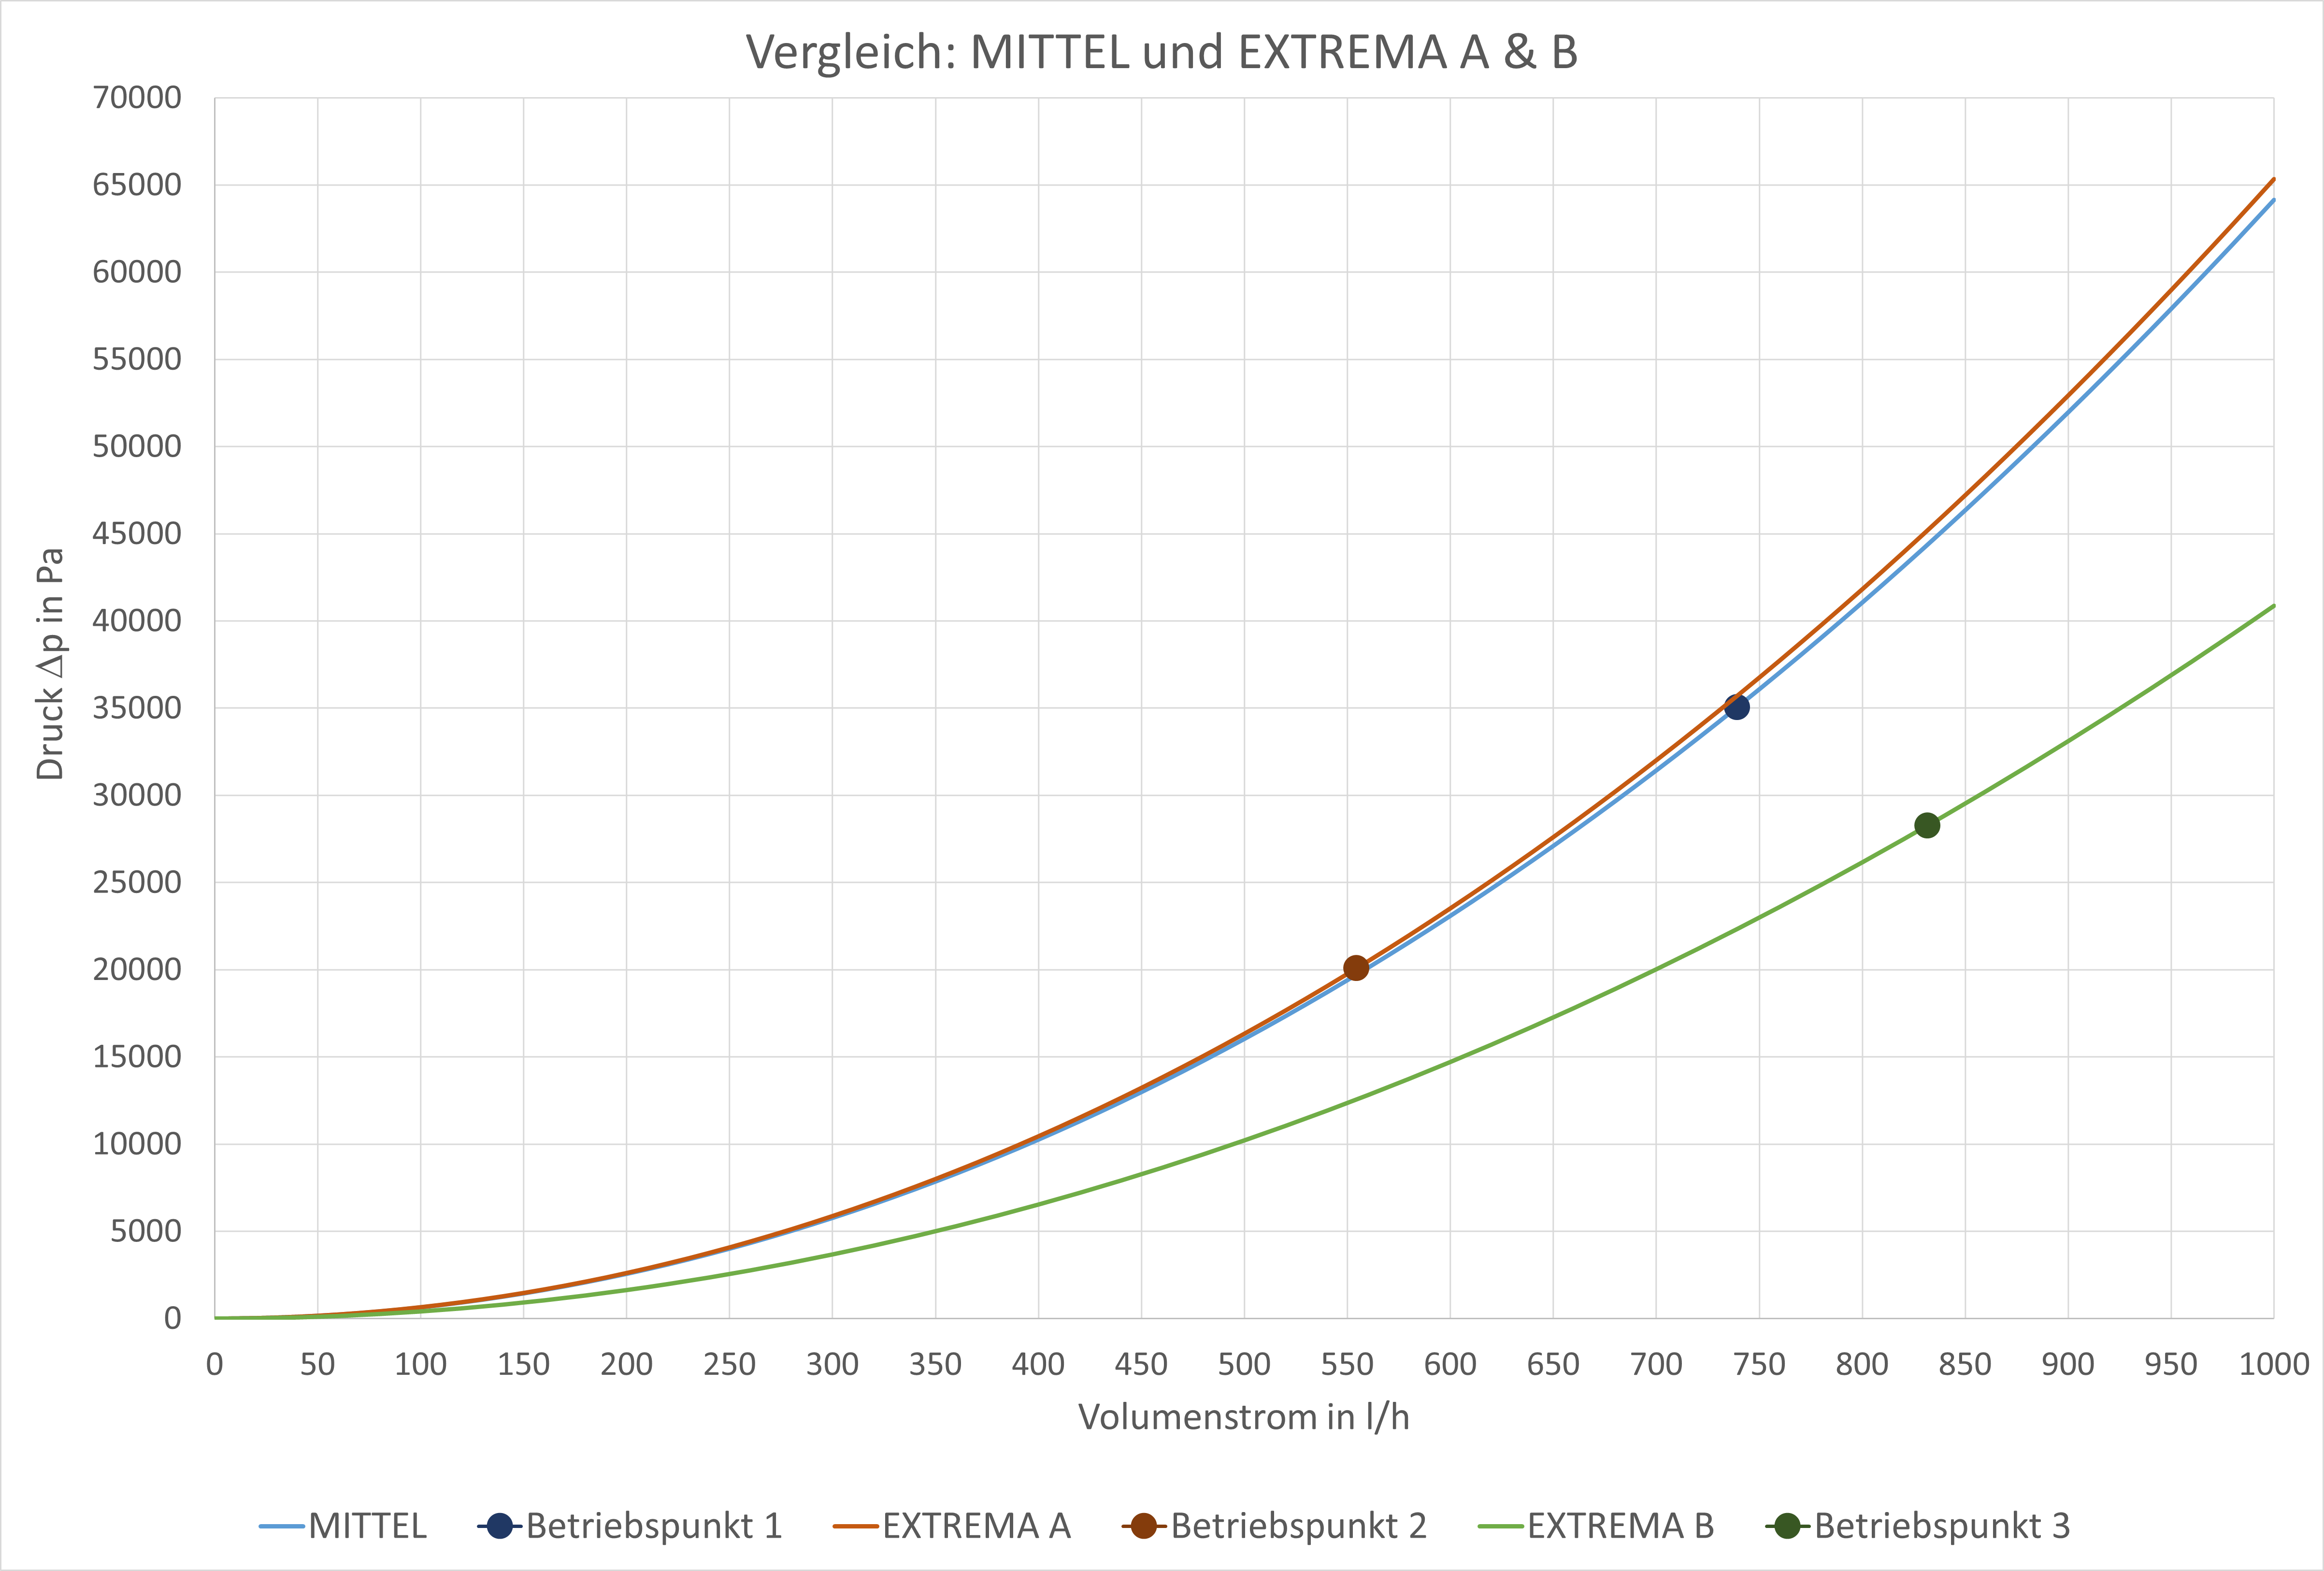
\includegraphics[width=\textwidth]{Abbildungen/Kennlinie-Vergleich.png}
    \caption{Vergleich der Kennlinien und Betriebspunkte aller Auslegungen}
    \label{Vergleich}
\end{figure}

Abschließend würde ich das System an das zweite Extrema anpassen.
Denn trotz der Mehrkosten für Kollektoren und Verrohrung wäre dieses System gegenüber den beiden
Anderen finanziell vorteilhafter, da so sichergestellt werden kann, dass auch bei schlechten Umständen der
solare Deckungsgrad auf min. 30\% gehalten wird und so eine Inbetriebnahme der Nachheizung außerhalb
der Heizperioden verhindert werden könnte. Zusätzlich kann im Vergleich zum Mittel-System in \autoref{sec:Pumpe}
ein kleineres und entsprechend preiswerteres Pumpenmodell gewählt werden.
